\section{Imagina Juntos}
\label{imagine}

Uma vez em que estivermos rodando os nossos trabalhos no ``Estado de arte'', sobrará muito tempo livre para criarmos e inovamos. 

Por exemplo, imagine se a Hotmart fosse da seguinte maneira:
\begin{figure}[H]
    \centering
    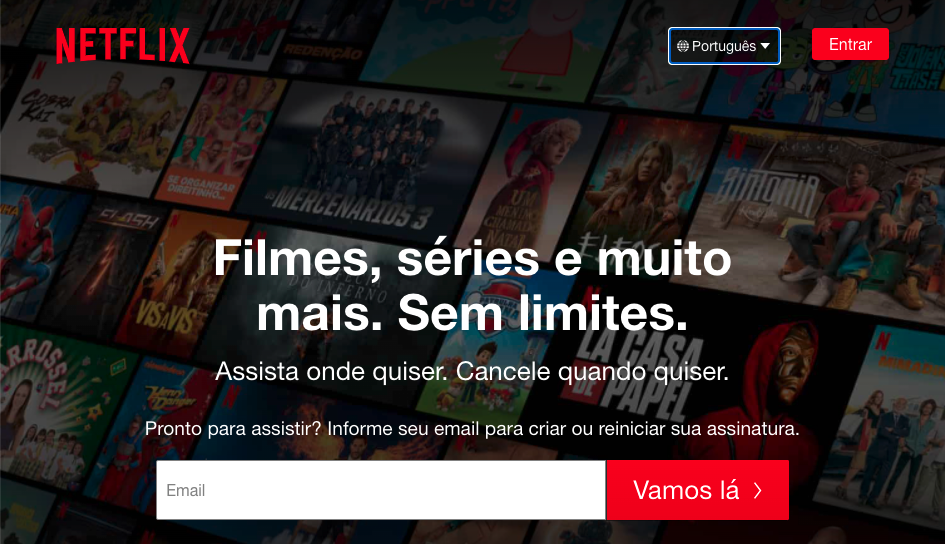
\includegraphics[scale=0.35,keepaspectratio=true]{images/04.png}
    \caption{Tela de login}
    \label{04}
\end{figure}

A Figura \ref{04}, seria uma tela de login bem simples, apenas para identificarmos o usuário e definirmos alguns parâmetro como idioma ou país para o qual devemos redirecionar o nosso vasto catálogo de produtos digitais. 
\begin{figure}[H]
    \centering
    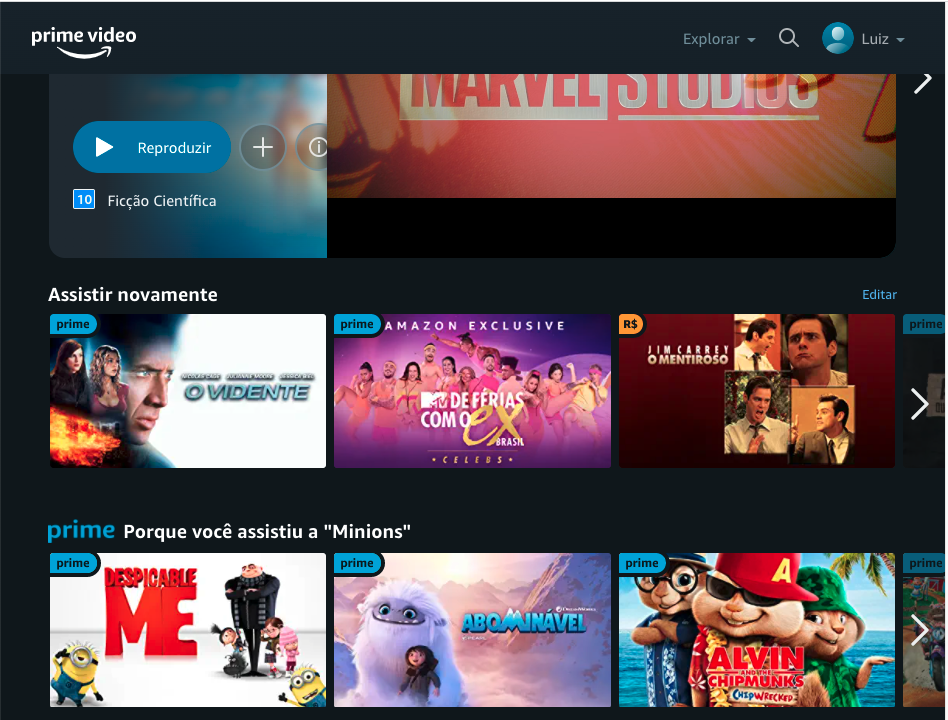
\includegraphics[scale=0.32,keepaspectratio=true]{images/05.png}
    \caption{Catálogo Hotmart -- conteúdo gratuito e pago ``on-demand''}
    \label{05}
\end{figure}

Na Figura \ref{05}, o usuário poderia se deparar com conteúdo gratuito, ou seja, trial, de vendedores que desejam que ele possa testar seu produto antes de comprar. Os compradores poderiam testar quantos produtos desejassem até que se decidam compar. Um vantagem é que como não haveria uma compra, não haveria solicitações de reembolso bem como tentativas de fraudes. O conteúdo gratuito poderia ser a primeira aula ou algum video para convencer o usuário a compar. 

\begin{figure}[H]
    \centering
    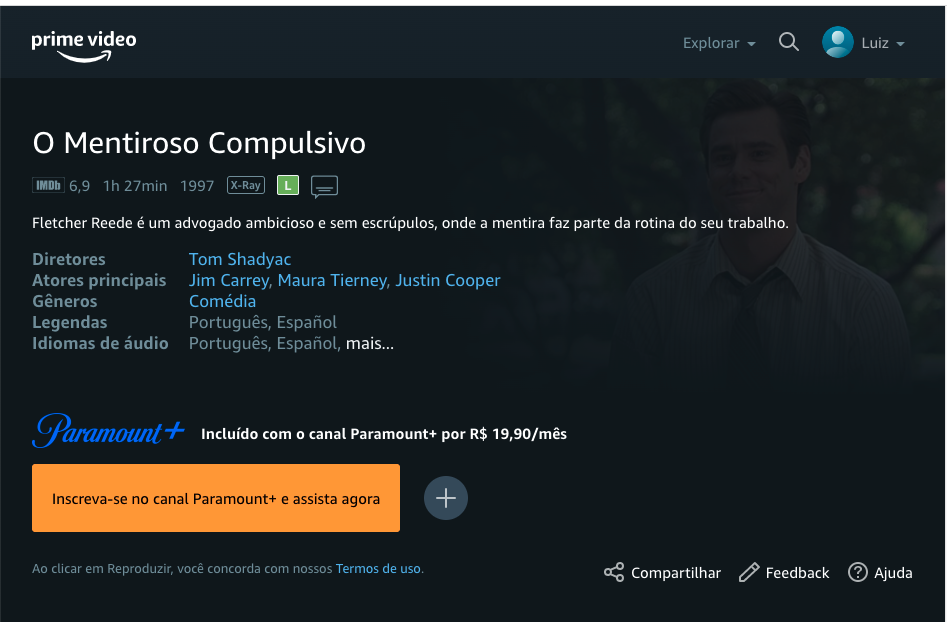
\includegraphics[scale=0.35,keepaspectratio=true]{images/06.png}
    \caption{Página de vendas}
    \label{06}
\end{figure}

Na Figura \ref{06} ilustra como seria a página de vendas de um produto. Neste momento, o vendedor configura sua oferta como bem entender: pagamento único, assinatura, smart installment, pagamento híbrido, etc. 

\begin{figure}[H]
    \centering
    
\includegraphics[scale=0.52,keepaspectratio=true]{images/07.png}
    \caption{Menus ao lado do ícone da Hotmart}
    \label{07}
\end{figure}
A Figura \ref{07} ilustra como seria interessante haver menus que transmitissem a mensagem de que a plataforma não é apenas para compras. Uma sugestão seria: COMPRAR - MINHAS COMPRAS - VENDER - MINHAS VENDAS - AJUDA